\documentclass{beamer}

%Packages BEGIN
\usepackage{amsmath}
\usepackage{xeCJK} % use this package to set Chinese and English font separately
\usepackage{fontspec} 
 

%Packages END

%Style setting BEGIN
\usetheme{Madrid} 
\usecolortheme{default} 

% Serif font in Ubuntu. Choose the Chinese font available in your device
\setCJKmainfont{Noto Serif CJK TC}

% Serif font in Ubuntu. Choose the Chinese font available in your device
\setCJKmonofont{Noto Serif CJK TC}

% Serif font in Ubuntu. Choose the Chinese font available in your device
\setCJKsansfont{Noto Serif CJK TC}

\XeTeXlinebreaklocale "zh" % enabling auto linebreaks
\XeTeXlinebreakskip = 0pt plus 1pt % enabling auto linebreaks
 
%Style setting END

\title{Anki Auto-lookup}
\subtitle{A convenient tool for English learning}
\author[張家翔, 王昊謙, 徐鼎翔]
{B08901062 張家翔\inst{1} \and 
B07202020 王昊謙\inst{2} \and 
B07202037 徐鼎翔 \inst{2}}
 
\institute[NTU] % (optional)
{
	\inst{1}%
	Department of Electrical Engineering\\
	National Taiwan University
	\and
	\inst{2}%
	Department of Physics\\
	National Taiwan University
} 

\begin{document}

\frame{\titlepage} 

\begin{frame}{Adding Cards}
	\textbf{Step1}: Connect with Anki API.\\
	\textbf{Step2}: Create a model that contains the fields we need.
	\begin{figure}[h]
			\centering
			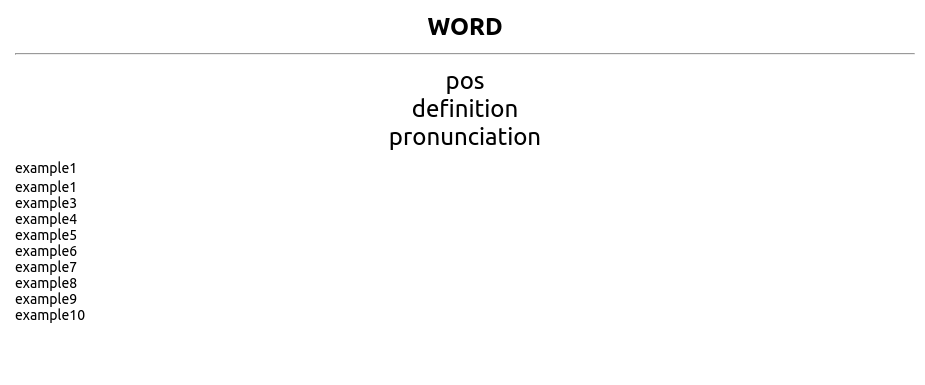
\includegraphics[width=1.00\linewidth]{./model_example.png}
	\end{figure}
\end{frame}

\begin{frame}{Adding Cards}
	\textbf{Step3}: Create a new card using the information got by the crawler.
	\begin{figure}[h]
			\centering
			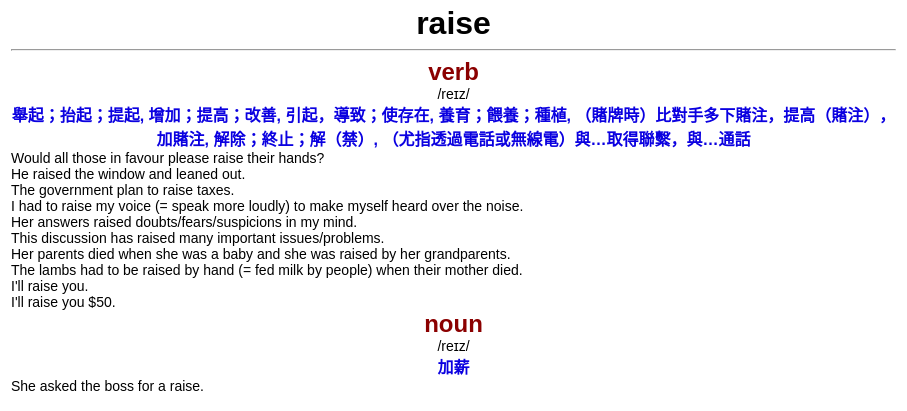
\includegraphics[width=1.0\linewidth]{./card_sample.png}
	\end{figure}
\end{frame}

\begin{frame}{GUI}
		\text Module: \textbf{tkinter}\\
		\text -Menu (select decks, select functions)\\
		\indent -Word Lookup\\
		\indent -Article Lookup\\
		\indent -Image Lookup\\
		\begin{figure}[h]
				\centering
				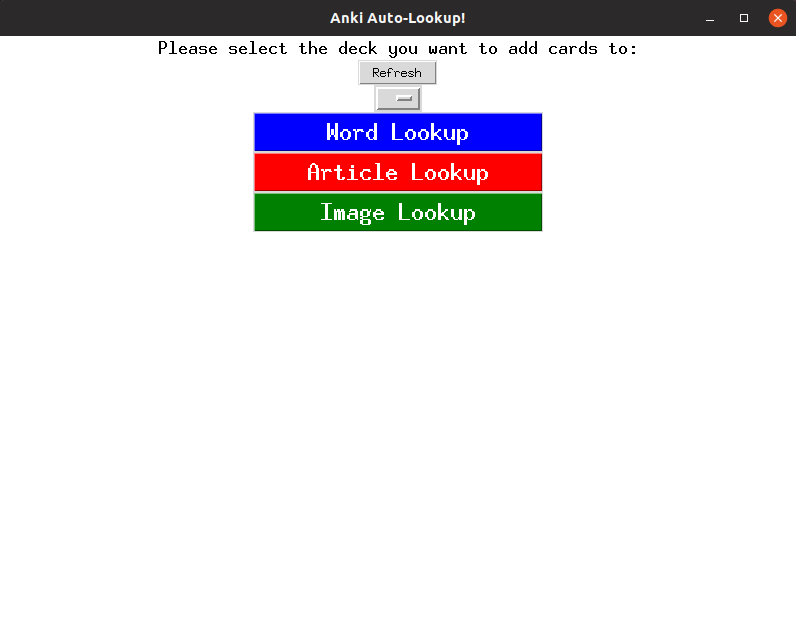
\includegraphics[width=0.6\linewidth]{./GUI_main.png}
		\end{figure}
\end{frame}

\begin{frame}{Word Lookup}
	\begin{enumerate}
		\item When you key in 'Enter', add the line into 'Words to be added' column.
		\item When you press 'Done', add the words into Anki.
	\end{enumerate}
	\begin{figure}[h]
			\centering
			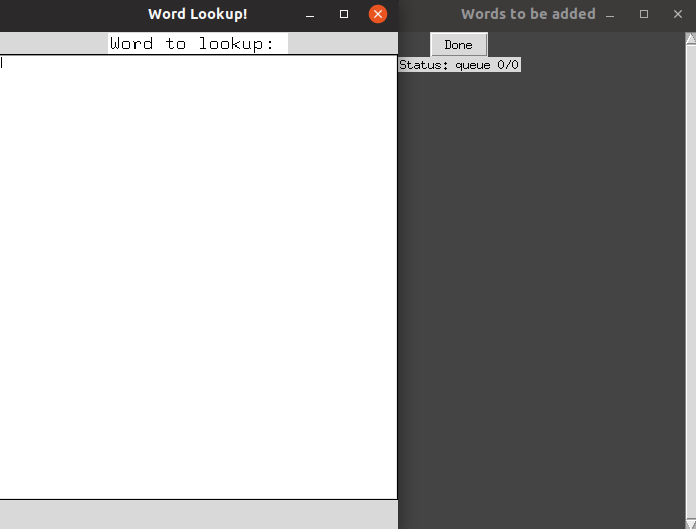
\includegraphics[width=0.6\linewidth]{./word_lookup_gui.png}
	\end{figure}
\end{frame}



\end{document}
